\documentclass[11pt]{article}
\usepackage{mypackages}
\begin{document}

\maketitle

\subsection{Using deep learning for approximating functions}

In the last section we claimed that a neural network could be used to approximate the
state-value and action-value functions.
When we refer to a neural network, what we mean is an artificial neural network -
a computational model that emulates connections between neurons in the human brain.
Formally this means that we wish to find the functions $v_\pi^{\sim}(s)$ and $q_\pi^{\sim}(s,a)$ that
satisfies $v_\pi^{\sim}(s) \approx v_\pi(s)$ and $q_\pi^{\sim}(s,a) \approx q_\pi(s, a)$.
In general this means that for a function $f(x)$, the neural network tries to approximate
$f^{\sim}(x)$ such that $f^{\sim}(x)$ varies the least from $f(x)$ for all $x$ in the input
space\cite{DeepLearningBook}.
It does so by adjusting its parameters based on experience - data for which $f(x)$ is already known -
that it can use to compute how well the current approximation is performing.

This data is exactly what is available to us in the agent-environtment model, when there is a natural terminal state,
since we can then use the experienced actual returns to update the weights of the models.

\subsubsection{Layers, neurons and connections}

The goal of deep learning is to separate difficult problems into smaller and simpler problems
and in this process create a hierarchy of concepts, where each concept can be described in terms
of simpler concepts\cite{DeepLearningBook}.

More formally, a neural network consists of \textit{layers} that each represent a concept, which
when connected are able to solve the complex problem at hand.
With this definition of a neural network the approximation function $f^{\sim}(x)$ can be
defined as
\begin{equation}
    f^{\sim}(x) = f^{k}(f^{k-1}( \cdots f^{0}(x) \cdots))
\end{equation}
for a network with $k$ layers.
The only layers that have their dimensions restrained are the first and last, since they are defined by the
dimensions of the input and the output of the approximator function.
This means the layers inbetween can have arbitrary shapes and
since we won't be seeing the output of those layers, we call them \textit{hidden layers}.
\begin{figure}[!h]
    \centering
    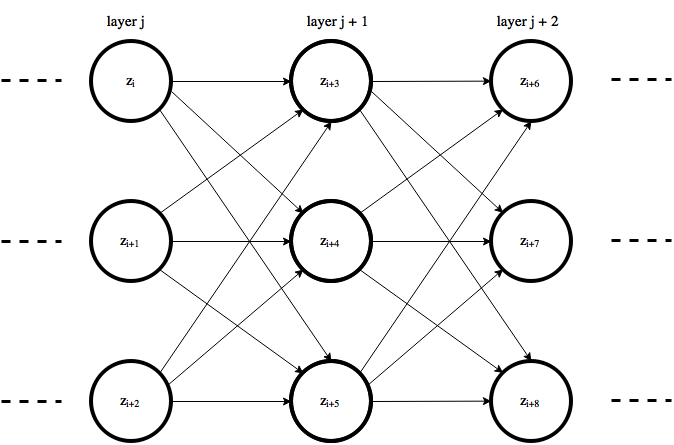
\includegraphics[width=10cm]{include/layers.png}
    \caption{A series of layers in a fully connected neural network.}
    \label{fig:layers}
\end{figure}
Each layer consists of a number of \textit{neurons} that are connected to the neurons of the
next layer.
%%%% Figure of layers

Each neuron transforms its series of input signals into a single output signal which is sent to
each neuron in the following layer through a \textit{weighted connection}, where
the weight of the connections define the importance of the signals.
Thus purpose of the hidden layers is to extract the key features of the original input.
They do so through the usage of \textit{activation functions}.
Activation functions take the weighted input signals and transform them
into a single output that describes a feature.
%%%% A drawing of a neuron “up close”
\begin{figure}[!h]
    \centering
    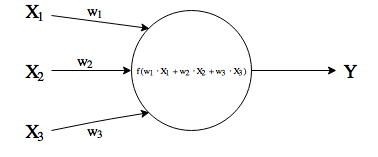
\includegraphics[width=10cm]{include/neuron.png}
    \caption{The structure of a single neuron with activation function $\alpha$.}
    \label{fig:neuron}
\end{figure}

This means that the role of the output of each layer is to provide some additional
transformation from the features in order to complete the task the network
must perform\cite{DeepLearningBook}.

\subsubsection{Learning from multidimensional input}

To process the high dimensional frames the Atari games we will be using
\textit{convolutional} layers.
We use convolutional layers to reduce the dimensionality of the
input frames and in that process extract important features of each frame.
To accomplish this a convolutional layer perform a \textit{convolution} over
its input.
A convolution is an operation on two functions, $a$ and $b$ that produces a third function
$h$ which is then the convolution of $a$ and $b$\cite{DeepLearningBook}.
The convolution operation is denoted by a $\ast$ and the convolution of $a$ and $b$
is formally defined as
\begin{equation}\label{eq:conv}
    (a \ast b)(x) = \int\limits_{-\infty}^{\infty} a(y) * b(x - y) dy
\end{equation}
where both $a$ and $b$ are continous.
The convolutions of the network are used on frames from the Atari games, which
means that they are applied to discrete sequences.

To accommodate for this we start by describing a convolution as a sum of infinite
discrete sequences.
This transforms equation \ref{eq:conv} into
\begin{equation}
    (a \ast b)(x) = \sum\limits_{y = -\infty}^{\infty} a(y) * b(x - y)
\end{equation}

Now what we really want is to apply convolutions to the frames from the Atari games.
These have a fixed size which means they are represented as \textbf{finite} sequences
so we extend the sequences by 0's to make them \textbf{infinite} whenever a convolution
is applied to a pixel “outside” of the frames.

In our network we can view the input images as a function $f : \R^{(x, y)} \to \R$ and
to extract the features of the image we apply a filter function $g : \R^{(d, d)} \to \R$
using a convolutoon.
This convolution can is then a neighbourhood operation, where each output pixel
is a weighted sum of its neighbouring pixels\cite{convSE}.
\begin{figure}[!h]
    \centering
    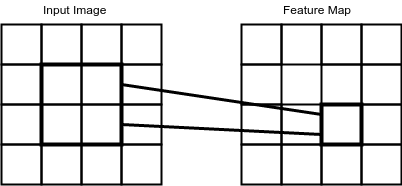
\includegraphics[width=10cm]{include/conv.png}
    \caption{A convolution on an input map which produces a \textit{feature} map.}
    \label{fig:conv}
\end{figure}

Using a convolution on an image produces a \textit{feature map}.
This feature map has the property that each of its elements is
the result of a convolution of the input with a linear filter\cite{DeepLearningBook}.
In the network, the filter function $g$ corresponds to a weight matrix $\mathbf{W}$ shared between all neurons in the layer.
$$
\mathbf{W} =
\begin{bmatrix}
    w_{1,1 } & w_{1, 2} & \hdots & w_{1, d} \\
    w_{2,1 } & w_{2, 2} & \hdots & w_{2, d} \\
    \vdots   &          & \ddots &          \\
    w_{d,1 } & w_{d, 2} & \hdots & w_{d, d} \\
\end{bmatrix}
$$

This means that there is as many neurons as there are elements in the feature map.
Each neuron can then be seen as a linear transformation given by
\begin{equation}
    X_{i, j} = \sum\limits_{z, q} W_{z, q} * X_{z, q}
\end{equation}
for all $z, q$ in the filter with center in $X_{i, j}$.

% Måske ændre fra raw til preproccessed
As explained in section \ref{Data} there are a lot of pixels in the raw Atari frames that
contain little information abut the state.
To reduce the amount of areas without relevance we have chosen to \textit{subsample}
the input images after they has gone through a convolution.


Now the convolution in itself doesn't reduce the dimensionality of its input


\subsubsection{Updating the weights using gradients}

A neural network is trained to minimize its total loss based on its \textit{loss
function}.
A loss function $\mathcal{L} : \R^K \to \R$ is supposed to describe how close the
predictions are to the true result.
In the reinforcement learning setting it is often difficult to estimate the
true result.
E.g. for a policy aproximator $\pi^{\sim}(A_t | S_t)$ we want to use the knowledge
of wether or not action $A_t$ was  chosen in state $S_t$ to determine
whether the probability of taking $A_t$ should be increased or decreased to
reduce the loss of the network.
Therefore the weights of the connections in the network are typically updated
in a direction in the weight space.
This direction describes how the weights should be updated to increases the
probability of repeating the action $A_t$ the most on future visits to
state $S_t$\cite{RLbook}.
To find the direction we would use the \textit{gradient} of the probability of
taking the action actually taken, since it exactly describes how to increate
this probability.

Now, this would increase the chance of picking action $A_t$ in state $S_t$ again,
but we really only want to pick actions again that lead to a good return.
Therefore the probability is generally updated proportionally to the
return, since the network will then learn to favor actions that provide
the highest return.


\end{document}
